% Bagian Lampiran
\section*{Lampiran} % Jika ada lampiran

% ini buat percobaan 1

\begin{figure}[H]
  \centering
  % Kalau mau menambah gambar lagi tinggal nambahin begin{subfigure} -> end{subfigure}
  \begin{subfigure}[c]{0.4\linewidth}
    \centering
    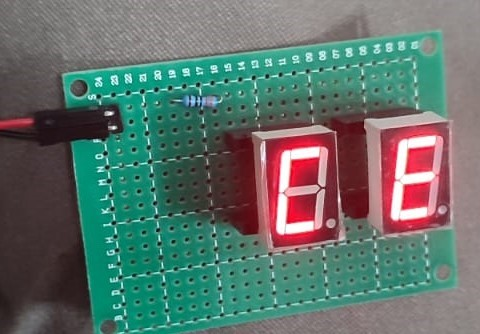
\includegraphics[width=\linewidth]{img/modul_2/percobaan1_hasil.jpg}
    \caption{Hasil 7 segment saat dinyalakan\label{fig:inisub1}}
  \end{subfigure}
  \hspace{1cm}
  \begin{subfigure}[c]{0.4\linewidth}
    \centering
    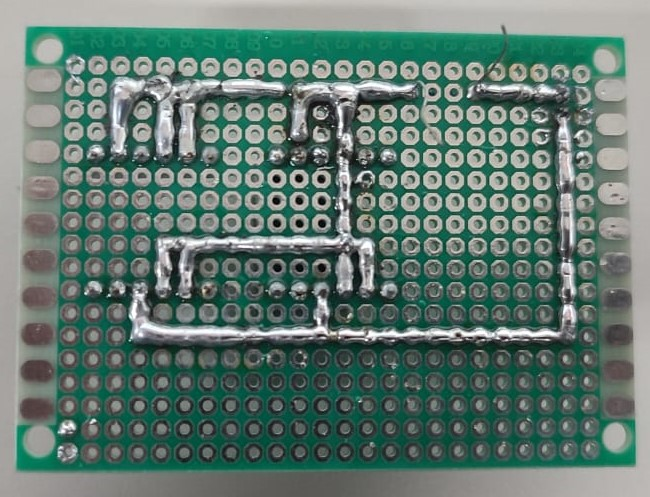
\includegraphics[width=\linewidth]{img/modul_2/percobaan1_hasil_solder.jpg}
    \caption{Hasil soldering PCB (tampak belakang) \label{fig:inisub2}}
  \end{subfigure}
  \caption{Hasil percobaan 1 \label{fig:keduagambar}}
\end{figure}

\begin{figure}[H]
  \centering
  % Kalau mau menambah gambar lagi tinggal nambahin begin{subfigure} -> end{subfigure}
  \begin{subfigure}[c]{0.4\linewidth}
    \centering
    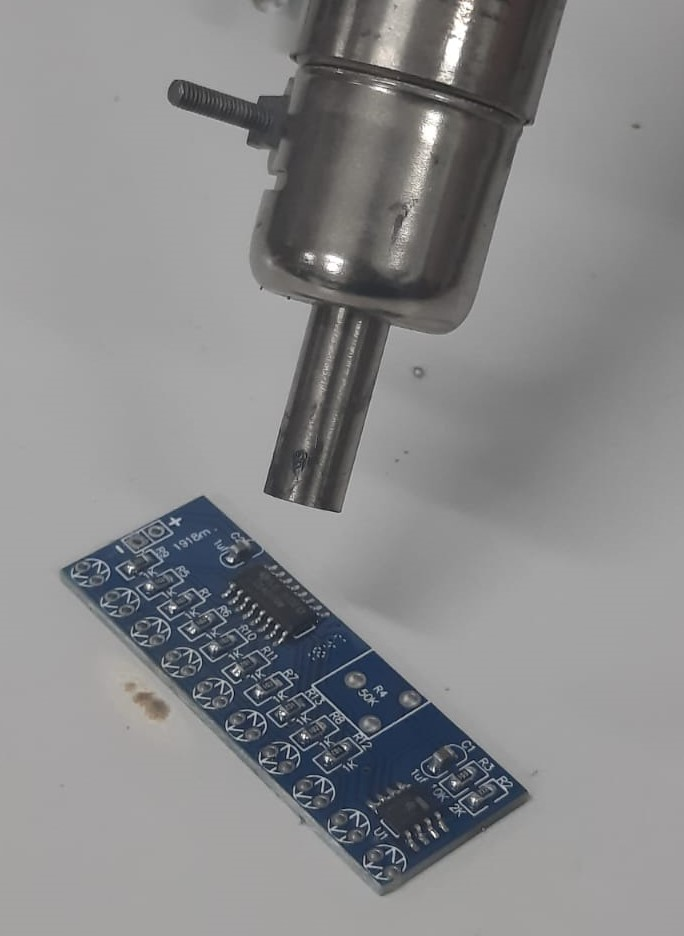
\includegraphics[width=\linewidth]{img/modul_2/percobaan2_soldering_uap.jpg}
    \caption{Proses soldering PCB menggunakan solder uap \label{fig:inisub1}}
  \end{subfigure}
  \hspace{1cm}
  \begin{subfigure}[c]{0.4\linewidth}
    \centering
    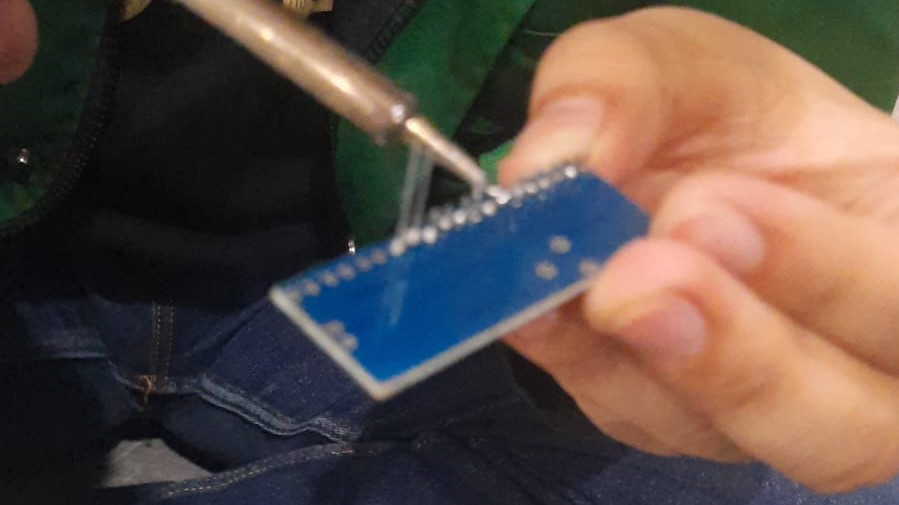
\includegraphics[width=\linewidth]{img/modul_2/percobaan2_soldering_biasa.jpg}
    \caption{Proses soldering PCB menggunakan solder biasa \label{fig:inisub2}}
  \end{subfigure}
  \caption{Proses soldering pada komponen percobaan 2 \label{fig:keduagambar}}
\end{figure}

\begin{figure}[H]
  \centering
  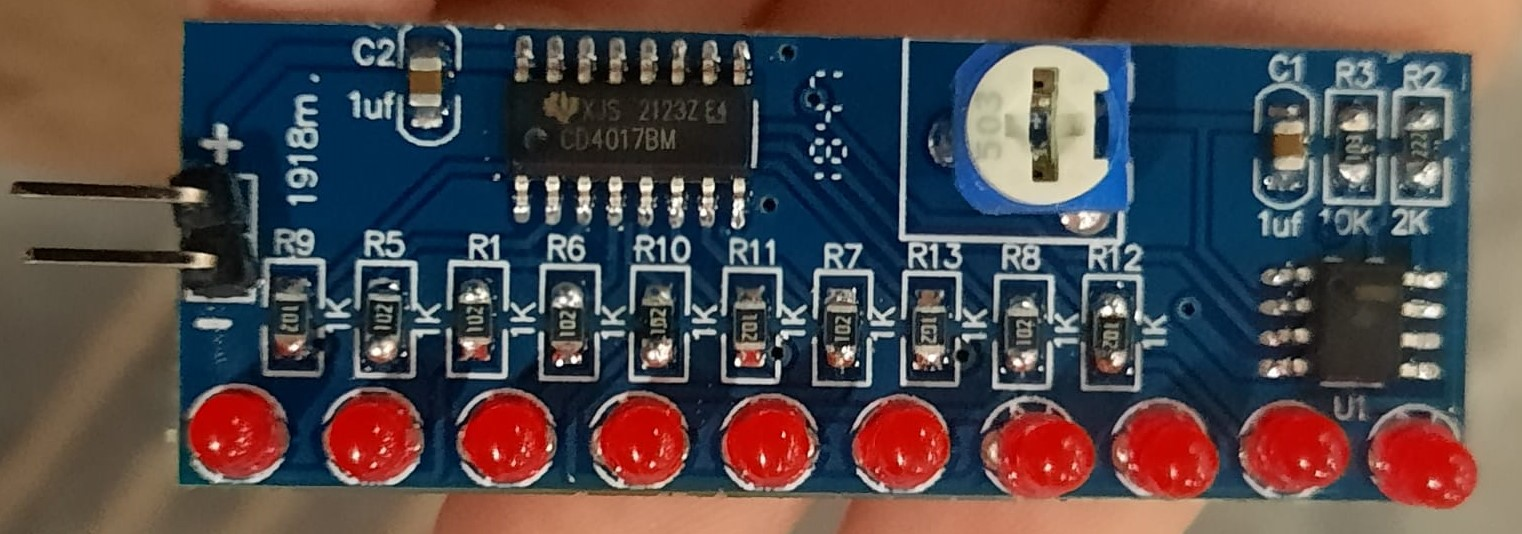
\includegraphics[width=0.7\linewidth]{img/modul_2/percobaan2_hasil.jpg}
  \caption{Hasil percobaan 2 \label{fig:inisub1}}
\end{figure}